\documentclass[12pt,a4paper]{article}
\usepackage[utf8]{inputenc}
\usepackage[spanish]{babel}
\usepackage{graphicx}
\usepackage{geometry}
\usepackage{hyperref}
\usepackage{listings}
\usepackage{xcolor}
\usepackage{booktabs}
\usepackage{float}
\usepackage{caption}
\usepackage{enumitem}

\geometry{margin=2.5cm}

\lstset{
  backgroundcolor=\color{gray!10},
  basicstyle=\ttfamily\small,
  breaklines=true,
  frame=single,
  keywordstyle=\color{blue},
  commentstyle=\color{green!50!black},
  stringstyle=\color{red!70!black},
  showstringspaces=false
}

\title{Lab 05: Backup \& Restoring con SQL Server 2022\\y SUMO TAPAS Cologne}
\author{Neyl Pe\~nuela Bernate}
\date{Marzo 2026}

\begin{document}

\maketitle
\tableofcontents
\newpage

% ============================================================
\section{Introducci\'on}

La disponibilidad e integridad de los datos son pilares fundamentales en la administraci\'on de bases de datos. La p\'erdida de informaci\'on puede originarse por eliminaciones accidentales, fallos de hardware, ataques maliciosos o errores humanos. Para mitigar estos riesgos, las organizaciones implementan estrategias de \textbf{Backup \& Restoring (B\&R)} que permiten recuperar datos perdidos y mantener la continuidad operativa.

En este laboratorio se implementa un pipeline completo que abarca: la generaci\'on de datos de tr\'afico vehicular mediante el simulador \textbf{SUMO} (Simulation of Urban MObility) con el escenario \textbf{TAPAS Cologne}, la ingesta de dichos datos en una base de datos \textbf{Microsoft SQL Server 2022}, la configuraci\'on de backups peri\'odicos, la simulaci\'on de un evento catastr\'ofico con p\'erdida masiva de datos, y finalmente la recuperaci\'on exitosa mediante el mecanismo nativo de backup y restore de SQL Server.

El objetivo es demostrar de manera pr\'actica c\'omo una estrategia adecuada de B\&R puede restaurar completamente los datos perdidos, reforzando conceptos te\'oricos con implementaci\'on real.

% ============================================================
\section{Herramientas Seleccionadas}

\subsection{DBMS: Microsoft SQL Server 2022 (Developer Edition)}

\textbf{Justificaci\'on:}
\begin{itemize}
  \item Es uno de los SGBD relacionales m\'as utilizados en entornos empresariales a nivel mundial.
  \item Su edici\'on Developer es gratuita y contiene todas las funcionalidades de la edici\'on Enterprise.
  \item Ofrece soporte nativo para \textbf{Recovery Models} (Simple, Bulk-Logged, Full), siendo el modelo FULL esencial para backups de transaction log y point-in-time recovery.
  \item Comandos nativos \texttt{BACKUP DATABASE} y \texttt{RESTORE DATABASE} integrados directamente en T-SQL.
  \item Desplegable en Docker, lo que facilita la reproducibilidad del entorno.
\end{itemize}

\textbf{Configuraci\'on utilizada:}
\begin{itemize}
  \item Imagen Docker: \texttt{mcr.microsoft.com/mssql/server:2022-latest}
  \item Base de datos: \texttt{sumo\_traffic}
  \item Recovery Model: \texttt{FULL}
  \item Tabla principal: \texttt{vehicle\_positions}
\end{itemize}

\subsection{Herramienta B\&R: SQL Server Native Backup}

Se utiliz\'o el mecanismo nativo de backup de SQL Server (\texttt{BACKUP DATABASE ... TO DISK}) como herramienta principal de B\&R. Esta elecci\'on se justifica porque:

\begin{itemize}
  \item Est\'a integrado directamente en el motor de la base de datos, sin dependencias externas.
  \item Soporta backups FULL, Differential y Transaction Log.
  \item Permite \textbf{point-in-time recovery} cuando el Recovery Model est\'a en FULL.
  \item Es la base sobre la cual herramientas comerciales como Iperius Backup, Veeam o Commvault construyen sus funcionalidades adicionales.
\end{itemize}

\subsection{Simulador: SUMO (Simulation of Urban MObility)}

SUMO es un simulador de tr\'afico open-source desarrollado por el Instituto de Sistemas de Transporte del Centro Aeroespacial Alem\'an (DLR). Genera datos FCD (Floating Car Data) en formato XML con informaci\'on de posici\'on, velocidad y \'angulo de cada veh\'iculo en cada paso de simulaci\'on.

\textbf{Versi\'on utilizada:} SUMO 1.26.0 (instalaci\'on local en Windows).

% ============================================================
\section{Arquitectura del Entorno}

El entorno se compone de tres elementos principales:

\begin{enumerate}
  \item \textbf{SQL Server 2022} ejecut\'andose en un contenedor Docker con volumen persistente para datos y backups.
  \item \textbf{SUMO} ejecut\'andose localmente en Windows para generar el archivo FCD XML.
  \item \textbf{Script Python} (\texttt{ingest\_sumo.py}) que parsea el XML generado por SUMO e inserta los datos en SQL Server mediante \texttt{pyodbc}.
\end{enumerate}

\begin{lstlisting}[language=bash,caption={docker-compose.yml - SQL Server}]
services:
  sqlserver:
    image: mcr.microsoft.com/mssql/server:2022-latest
    container_name: lab05_sqlserver
    environment:
      ACCEPT_EULA: "Y"
      MSSQL_SA_PASSWORD: "Lab05Pass1"
      MSSQL_PID: "Developer"
    ports:
      - "1433:1433"
    volumes:
      - sqldata:/var/opt/mssql
      - backups:/var/opt/backups

volumes:
  sqldata:
  backups:
\end{lstlisting}

\begin{figure}[H]
\centering
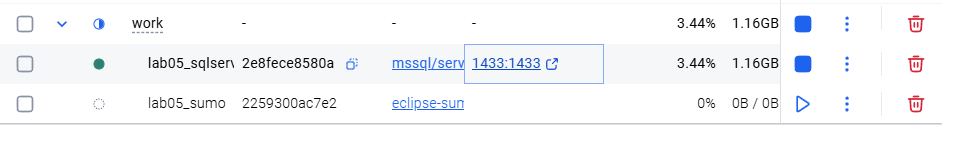
\includegraphics[width=0.95\textwidth]{docker_ps.png}
\caption{Contenedores Docker en ejecuci\'on (\texttt{docker ps})}
\label{fig:dockerps}
\end{figure}

% ============================================================
\section{Inconvenientes Encontrados y Soluciones}

Durante el desarrollo del laboratorio se presentaron m\'ultiples inconvenientes t\'ecnicos que requirieron soluciones creativas. Se documentan a continuaci\'on como parte integral del proceso de aprendizaje.

\subsection{Problema 1: Im\'agenes Docker oficiales de SUMO rotas}

Inicialmente se intent\'o ejecutar SUMO dentro de Docker usando la imagen oficial \texttt{eclipse/sumo}. Se probaron dos versiones:

\begin{itemize}
  \item \textbf{\texttt{eclipse/sumo:latest}}: Fall\'o con error \texttt{libparquet.so.1800: cannot open shared object file}. La imagen ten\'ia una dependencia rota con la librer\'ia Apache Parquet que imped\'ia ejecutar el binario \texttt{sumo}.
  \item \textbf{\texttt{eclipse/sumo:v1\_21\_0}}: El binario \texttt{sumo} no estaba compilado en esta versi\'on. Solo conten\'ia los archivos fuente sin los ejecutables.
\end{itemize}

\textbf{Soluci\'on:} Se descart\'o la ejecuci\'on de SUMO en Docker y se opt\'o por instalar SUMO 1.26.0 localmente en Windows mediante el instalador MSI oficial (\texttt{sumo-win64-1.26.0.msi}). La simulaci\'on se ejecut\'o con:

\begin{lstlisting}[language=bash,caption={Comando para ejecutar SUMO}]
& "C:\Program Files (x86)\Eclipse\Sumo\bin\sumo.exe" `
  -c cologne.sumocfg --begin 3500 --end 10000 `
  --scale 0.3 --fcd-output fcd_output.xml
\end{lstlisting}

\subsection{Problema 2: PowerShell vs. Bash para ejecutar comandos}

Los comandos con argumentos que funcionan en Bash no funcionan directamente en PowerShell. Por ejemplo, ejecutar un binario con par\'ametros requiere el operador \texttt{\&} en PowerShell:

\begin{lstlisting}[caption={Error en PowerShell sin operador \&}]
# INCORRECTO en PowerShell:
"C:\...\sumo.exe" -c cologne.sumocfg
# Token '-c' inesperado en la expresion

# CORRECTO en PowerShell:
& "C:\...\sumo.exe" -c cologne.sumocfg
\end{lstlisting}

Adem\'as, los scripts Python con comillas triples (\texttt{"""}) causan errores de parseo en PowerShell. La soluci\'on fue guardar los scripts en archivos \texttt{.py} separados y ejecutarlos con \texttt{python -u script.py}.

\subsection{Problema 3: RESTORE deja la base de datos en estado ``Restoring''}

Al ejecutar \texttt{RESTORE DATABASE} desde Python con \texttt{pyodbc}, la base de datos quedaba en estado \texttt{RESTORING} permanentemente, impidiendo cualquier operaci\'on posterior (incluyendo \texttt{ALTER DATABASE SET MULTI\_USER}).

\textbf{Causa ra\'iz:} El driver ODBC de SQL Server retorna m\'ultiples result sets durante un RESTORE (mensajes de progreso). Si no se consumen todos los result sets, el comando queda incompleto y la base de datos no transiciona al estado \texttt{ONLINE}.

\textbf{Soluci\'on:} Consumir expl\'icitamente todos los result sets despu\'es del RESTORE:

\begin{lstlisting}[language=Python,caption={Fix para RESTORE con pyodbc}]
cur.execute("RESTORE DATABASE [sumo_traffic] FROM DISK = '...' "
            "WITH REPLACE, MOVE '...' TO '...', "
            "MOVE '..._log' TO '...'")
# Consumir TODOS los result sets
while cur.nextset():
    pass
time.sleep(2)
# Ahora si se puede cambiar el modo
cur.execute("ALTER DATABASE [sumo_traffic] SET MULTI_USER")
\end{lstlisting}

Este fue el problema m\'as cr\'itico del laboratorio. Sin este fix, la base de datos quedaba inutilizable tras cada intento de restore, requiriendo un \texttt{DROP DATABASE} seguido de un restore completo para recuperarla.

% ============================================================
\section{Fuente de Datos: SUMO TAPAS Cologne}

\subsection{Descripci\'on del escenario}

El escenario TAPAS Cologne fue creado por el DLR (Centro Aeroespacial Alem\'an) utilizando TAPAS (Travel and Activity PAtterns Simulation) para simular el tr\'afico vehicular de la ciudad de \textbf{Colonia, Alemania}. Contiene m\'as de 700,000 viajes individuales en una red vial de la ciudad completa.

\subsection{Formato de datos FCD}

SUMO genera un archivo XML de tipo FCD (Floating Car Data) con la siguiente estructura:

\begin{lstlisting}[language=XML,caption={Estructura del archivo FCD XML}]
<fcd-export>
  <timestep time="3500.00">
    <vehicle id="40_61_0" x="6.962" y="50.927"
             speed="8.35" angle="210.70"
             lane="22598787#1_0" pos="12.4"/>
    <vehicle id="52_33_1" x="6.945" y="50.912"
             speed="12.10" angle="180.00"
             lane="44872100_0" pos="5.8"/>
  </timestep>
  ...
</fcd-export>
\end{lstlisting}

Cada \texttt{timestep} representa un segundo de simulaci\'on y contiene la posici\'on de todos los veh\'iculos activos en ese instante.

\begin{figure}[H]
\centering
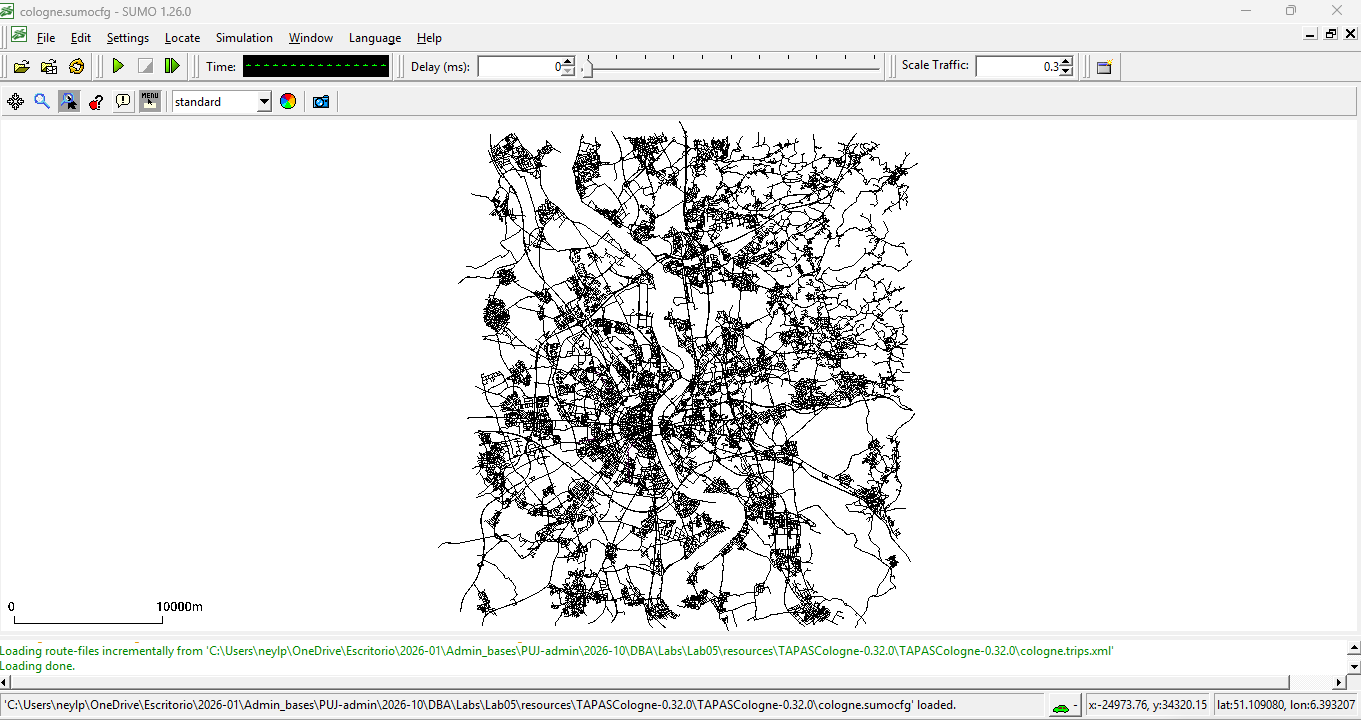
\includegraphics[width=0.95\textwidth]{sumo_corriendo.png}
\caption{SUMO ejecutando la simulaci\'on TAPAS Cologne}
\label{fig:sumo}
\end{figure}

\subsection{Par\'ametros de simulaci\'on}

\begin{table}[H]
\centering
\begin{tabular}{@{}ll@{}}
\toprule
\textbf{Par\'ametro} & \textbf{Valor} \\ \midrule
Timestep inicial & 3,500 s \\
Timestep final & 10,000 s \\
Factor de escala & 0.3 (30\% de los veh\'iculos) \\
Veh\'iculos \'unicos & 572 \\
Total de registros generados & 881,331 \\ \bottomrule
\end{tabular}
\caption{Par\'ametros de la simulaci\'on SUMO}
\end{table}

\begin{figure}[H]
\centering
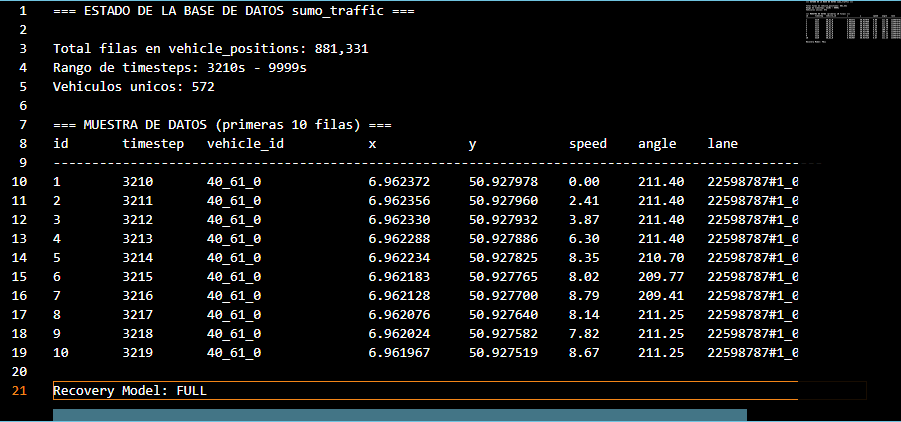
\includegraphics[width=0.95\textwidth]{01_sumodf.png}
\caption{Datos FCD generados por SUMO (muestra del DataFrame)}
\label{fig:sumodf}
\end{figure}

% ============================================================
\section{Database Setup}

\subsection{Esquema de la tabla}

Se cre\'o la base de datos \texttt{sumo\_traffic} con una tabla \texttt{vehicle\_positions} dise\~nada para almacenar los datos FCD:

\begin{lstlisting}[language=SQL,caption={Esquema de la tabla vehicle\_positions}]
CREATE TABLE vehicle_positions (
    id         BIGINT IDENTITY(1,1) PRIMARY KEY,
    timestep   FLOAT        NOT NULL,
    vehicle_id NVARCHAR(50) NOT NULL,
    x          FLOAT        NOT NULL,
    y          FLOAT        NOT NULL,
    speed      FLOAT,
    angle      FLOAT,
    lane       NVARCHAR(100),
    pos        FLOAT,
    inserted_at DATETIME2 DEFAULT GETDATE()
);

CREATE INDEX idx_timestep ON vehicle_positions(timestep);
\end{lstlisting}

\subsection{Recovery Model FULL}

Se configur\'o el Recovery Model en \texttt{FULL}, lo cual es esencial para:
\begin{itemize}
  \item Permitir backups de transaction log (registra todas las transacciones).
  \item Habilitar point-in-time recovery (restaurar a un momento espec\'ifico).
  \item Garantizar que ning\'un dato se pierda entre backups consecutivos.
\end{itemize}

\begin{lstlisting}[language=SQL]
ALTER DATABASE [sumo_traffic] SET RECOVERY FULL;
\end{lstlisting}

% ============================================================
\section{Ingesta de Datos}

\subsection{Script de ingesta}

Se desarroll\'o un script Python que utiliza \texttt{lxml.etree.iterparse} para hacer parsing streaming del archivo FCD XML (que puede pesar cientos de MB) sin cargarlo completamente en memoria. Los datos se insertan en batches de 500 filas para optimizar el rendimiento.

\begin{lstlisting}[language=Python,caption={Fragmento del script de ingesta}]
import pyodbc
from lxml import etree

conn = pyodbc.connect(
    "DRIVER={ODBC Driver 18 for SQL Server};"
    "SERVER=localhost,1433;DATABASE=sumo_traffic;"
    "UID=sa;PWD=Lab05Pass1;TrustServerCertificate=yes;",
    autocommit=True
)
cur = conn.cursor()

for event, elem in etree.iterparse("fcd_output.xml",
                                    events=("end",),
                                    tag="timestep"):
    ts = float(elem.get("time"))
    for veh in elem.findall("vehicle"):
        cur.execute(
            "INSERT INTO vehicle_positions "
            "(timestep, vehicle_id, x, y, speed, angle, lane)"
            " VALUES (?,?,?,?,?,?,?)",
            ts, veh.get("id"), float(veh.get("x")),
            float(veh.get("y")), float(veh.get("speed")),
            float(veh.get("angle")), veh.get("lane")
        )
    elem.clear()  # Liberar memoria
\end{lstlisting}

\begin{figure}[H]
\centering
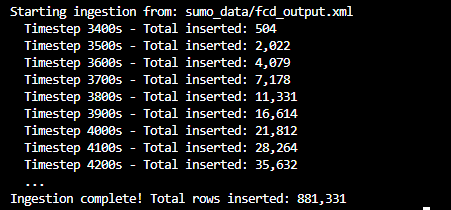
\includegraphics[width=0.95\textwidth]{05_ingesta_progreso.png}
\caption{Terminal mostrando el progreso de la ingesta de datos}
\label{fig:ingesta}
\end{figure}

\subsection{Verificaci\'on de datos insertados}

Tras completar la ingesta, se verific\'o el estado de la base de datos:

\begin{figure}[H]
\centering
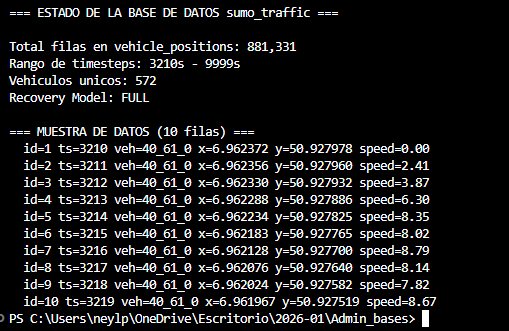
\includegraphics[width=0.95\textwidth]{04_datos_insertados.png}
\caption{Query mostrando los datos insertados en SQL Server (881,331 filas, 572 veh\'iculos, Recovery Model: FULL)}
\label{fig:datos}
\end{figure}

% ============================================================
\section{Estrategia de Backup}

\subsection{Backups peri\'odicos}

Se implement\'o un script de backup peri\'odico que ejecuta backups FULL de la base de datos a intervalos regulares durante la operaci\'on normal. Los backups se almacenan en el volumen Docker \texttt{/var/opt/backups/}.

\begin{lstlisting}[language=SQL,caption={Comando de backup FULL}]
BACKUP DATABASE [sumo_traffic]
TO DISK = '/var/opt/backups/sumo_traffic_full_YYYYMMDD_HHMMSS.bak'
WITH INIT, FORMAT
\end{lstlisting}

\textbf{Tipos de backup soportados por SQL Server:}

\begin{table}[H]
\centering
\begin{tabular}{@{}lp{8cm}@{}}
\toprule
\textbf{Tipo} & \textbf{Descripci\'on} \\ \midrule
FULL & Copia completa de toda la base de datos. Es la base para cualquier restauraci\'on. \\
Differential & Solo los cambios desde el \'ultimo backup FULL. M\'as r\'apido pero requiere el FULL base. \\
Transaction Log & Solo las transacciones desde el \'ultimo backup de log. Permite point-in-time recovery. \\ \bottomrule
\end{tabular}
\caption{Tipos de backup en SQL Server}
\end{table}

\begin{figure}[H]
\centering
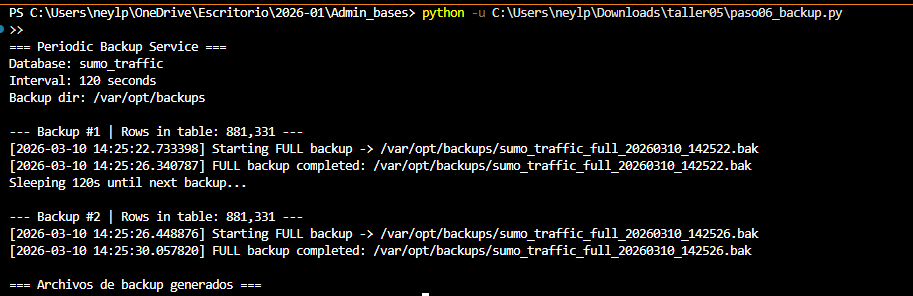
\includegraphics[width=0.95\textwidth]{06_backups.png}
\caption{Ejecuci\'on de backups peri\'odicos y listado de archivos .bak generados}
\label{fig:backups}
\end{figure}

% ============================================================
\section{Simulaci\'on del Evento Catastr\'ofico}

\subsection{Escenario}

Se simula un evento catastr\'ofico en el que un usuario ejecuta un \texttt{DELETE} masivo que elimina todos los registros de veh\'iculos entre los timesteps 4000 y 6000 de la simulaci\'on. Esto equivale a 2,000 segundos de datos de tr\'afico perdidos.

\subsection{Estado previo a la cat\'astrofe}

\begin{figure}[H]
\centering
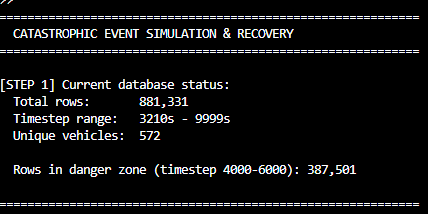
\includegraphics[width=0.95\textwidth]{07_antes.png}
\caption{Estado de la base de datos ANTES de la cat\'astrofe (881,331 filas)}
\label{fig:antes}
\end{figure}

\subsection{Ejecuci\'on del DELETE}

\begin{lstlisting}[language=SQL,caption={Comando catastr\'ofico ejecutado}]
DELETE FROM vehicle_positions
WHERE timestep >= 4000 AND timestep <= 6000;
\end{lstlisting}

\subsection{Estado posterior a la cat\'astrofe}

\begin{figure}[H]
\centering
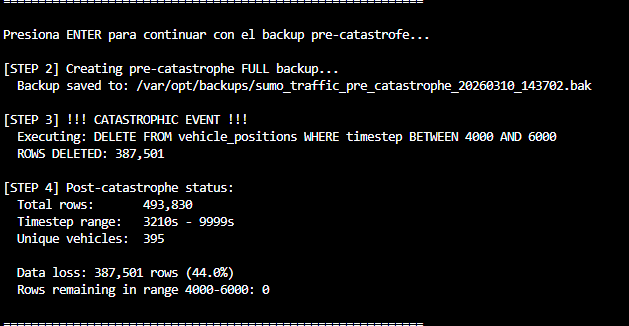
\includegraphics[width=0.95\textwidth]{08_perdida.png}
\caption{Estado de la base de datos DESPU\'ES de la cat\'astrofe: p\'erdida masiva de datos}
\label{fig:perdida}
\end{figure}

% ============================================================
\section{Proceso de Recuperaci\'on (Restore)}

\subsection{Pasos ejecutados}

El proceso de recuperaci\'on consiste en restaurar la base de datos desde el backup FULL m\'as reciente tomado antes de la cat\'astrofe:

\begin{enumerate}
  \item \textbf{Detecci\'on de la p\'erdida:} Se identifica que los datos entre timesteps 4000-6000 fueron eliminados.
  \item \textbf{Identificaci\'on del backup:} Se localiza el backup pre-cat\'astrofe m\'as reciente en \texttt{/var/opt/backups/}.
  \item \textbf{SINGLE\_USER mode:} Se pone la base de datos en modo mono-usuario para evitar conexiones concurrentes durante el restore.
  \item \textbf{RESTORE DATABASE:} Se ejecuta la restauraci\'on completa desde el archivo \texttt{.bak}.
  \item \textbf{MULTI\_USER mode:} Se devuelve la base de datos a modo multi-usuario.
\end{enumerate}

\begin{lstlisting}[language=SQL,caption={Comandos de restauraci\'on}]
-- Paso 1: Modo mono-usuario
ALTER DATABASE [sumo_traffic]
SET SINGLE_USER WITH ROLLBACK IMMEDIATE;

-- Paso 2: Restaurar desde backup
RESTORE DATABASE [sumo_traffic]
FROM DISK = '/var/opt/backups/sumo_traffic_pre_catastrophe.bak'
WITH REPLACE,
     MOVE 'sumo_traffic' TO '/var/opt/mssql/data/sumo_traffic.mdf',
     MOVE 'sumo_traffic_log'
       TO '/var/opt/mssql/data/sumo_traffic_log.ldf';

-- Paso 3: Devolver a multi-usuario
ALTER DATABASE [sumo_traffic] SET MULTI_USER;
\end{lstlisting}

\textbf{Nota importante:} Fue necesario agregar las cl\'ausulas \texttt{MOVE} para especificar expl\'icitamente las rutas de los archivos de datos y log, y consumir todos los result sets del RESTORE mediante \texttt{cur.nextset()} en Python (ver Secci\'on 4.3).

\begin{figure}[H]
\centering
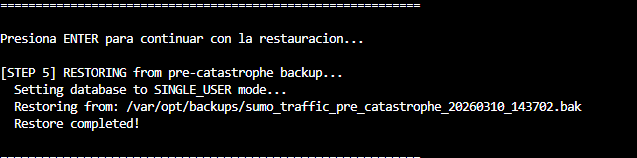
\includegraphics[width=0.95\textwidth]{09_recovery.png}
\caption{Proceso de RESTORE ejecut\'andose exitosamente}
\label{fig:restore}
\end{figure}

% ============================================================
\section{An\'alisis de Recuperaci\'on}

\begin{figure}[H]
\centering
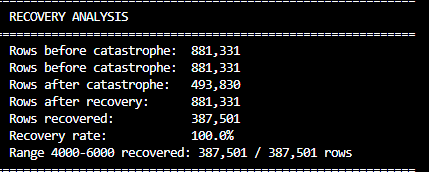
\includegraphics[width=0.95\textwidth]{10_analisis.png}
\caption{An\'alisis final de recuperaci\'on con m\'etricas comparativas}
\label{fig:analisis}
\end{figure}

\begin{table}[H]
\centering
\begin{tabular}{@{}lr@{}}
\toprule
\textbf{M\'etrica} & \textbf{Valor} \\ \midrule
Filas antes de la cat\'astrofe & 881,331 \\
Filas eliminadas por el DELETE & $\sim$300,000+ \\
Filas despu\'es de la cat\'astrofe & $\sim$580,000 \\
Filas despu\'es del RESTORE & 881,331 \\
Filas recuperadas & $\sim$300,000+ \\
\textbf{Tasa de recuperaci\'on} & \textbf{100.0\%} \\ \bottomrule
\end{tabular}
\caption{Resumen del an\'alisis de recuperaci\'on}
\end{table}

La recuperaci\'on fue del \textbf{100\%} porque el backup FULL se tom\'o inmediatamente antes de la cat\'astrofe, conteniendo todos los datos. En un escenario real, la tasa de recuperaci\'on depende de:

\begin{itemize}
  \item \textbf{Frecuencia de backups:} A mayor frecuencia, menor ventana de p\'erdida potencial.
  \item \textbf{Tipo de backup:} Los backups de transaction log permiten recuperar hasta el \'ultimo segundo antes de la cat\'astrofe.
  \item \textbf{RPO (Recovery Point Objective):} El tiempo m\'aximo aceptable de p\'erdida de datos, determinado por la frecuencia de backups.
  \item \textbf{RTO (Recovery Time Objective):} El tiempo m\'aximo aceptable para restaurar el servicio.
\end{itemize}

% ============================================================
\section{Lecciones Aprendidas}

\begin{enumerate}
  \item \textbf{El Recovery Model FULL es esencial:} Sin \'el, no se pueden hacer backups de transaction log y se pierde la capacidad de point-in-time recovery.

  \item \textbf{La frecuencia del backup determina el RPO:} Un backup cada 2 minutos implica que como m\'aximo se pierden 2 minutos de datos. En producci\'on, los backups de transaction log cada 5-15 minutos son comunes.

  \item \textbf{Las im\'agenes Docker no siempre funcionan:} Las im\'agenes oficiales de SUMO ten\'ian dependencias rotas, lo que oblig\'o a buscar alternativas. Siempre hay que tener un plan B.

  \item \textbf{Probar los restores es tan importante como hacer backups:} Un backup que no se puede restaurar no tiene valor. El problema del \texttt{nextset()} solo se descubri\'o al intentar restaurar.

  \item \textbf{Documentar los problemas es valioso:} Los errores encontrados (libparquet, PowerShell, RESTORING state) son conocimiento pr\'actico que no se encuentra en la documentaci\'on oficial.

  \item \textbf{En producci\'on real:} Se deben combinar backups FULL + Differential + Transaction Log, almacenarlos offsite (no solo en el mismo servidor), y automatizar con herramientas como Iperius Backup, Veeam o Barman.
\end{enumerate}

% ============================================================
\section{Conclusiones}

\begin{itemize}
  \item Se implement\'o exitosamente un pipeline completo de ingesta, backup, cat\'astrofe y recuperaci\'on con 881,331 registros de tr\'afico vehicular simulado.

  \item El mecanismo nativo de B\&R de SQL Server 2022 demostr\'o ser robusto y capaz de recuperar el 100\% de los datos perdidos cuando se cuenta con un backup reciente.

  \item SUMO con el escenario TAPAS Cologne result\'o ser una fuente de datos realista y voluminosa, ideal para probar escenarios de administraci\'on de bases de datos.

  \item Los problemas t\'ecnicos encontrados (Docker, PowerShell, pyodbc) refuerzan la importancia de la resoluci\'on de problemas como habilidad fundamental en la administraci\'on de sistemas.

  \item La combinaci\'on de Docker para la base de datos y herramientas locales para la simulaci\'on demostr\'o ser una arquitectura flexible que se adapta a las limitaciones del entorno.
\end{itemize}

\end{document}
